%%%%%%%%%%%%%%%%%%%%%%%%%%%%%%%%%%%%%%%%%%%%%%%%%%%%%%%%%%%%%%%%%%%%%%%%
%                                                                      %
%     File: Results/02_Missions.tex                                    %
%     Tex Master: ../Thesis.tex                                        %
%                                                                      %
%%%%%%%%%%%%%%%%%%%%%%%%%%%%%%%%%%%%%%%%%%%%%%%%%%%%%%%%%%%%%%%%%%%%%%%%

% ==============================================================================
\section{Missions}
\label{sec:res_missions}

% What do the missions add to the previous results?
The missions of Figure~\ref{fig:missions} put the manoeuvres together, with both vehicles moving at once and the manoeuvres of one waiting for the other. They test whether the two controllers, each driven by simple references, keep the system within its limits through a complete operation, from the takeoff to the landing, with the normal tether of $15\,\text{m}$. Each mission is shown in the same way. On the left, the paths of both vehicles are seen from above, with their positions and the tether at five instants, the older ones more transparent. On the right, the manoeuvres of each vehicle are shown over time, in their order in Figure~\ref{fig:missions}, together with the separation between the vehicles and the height of the \gls{uav}.

\subsection{Scout}
\label{subsec:res_scout}

% What does the scout show?
In the scout, the \gls{usv} sails a route of three legs at $1\,\text{m/s}$, with two turns of $90^\circ$, while the \gls{uav} flies $8\,\text{m}$ ahead of its bow and $5\,\text{m}$ above the winch, in the axes of the \gls{usv}, so that it turns with it and keeps looking ahead. The \gls{usv} sets off once the \gls{uav} is in its place, and the \gls{uav} lands when the route is over.

\begin{figure}[htbp]
    \centering
    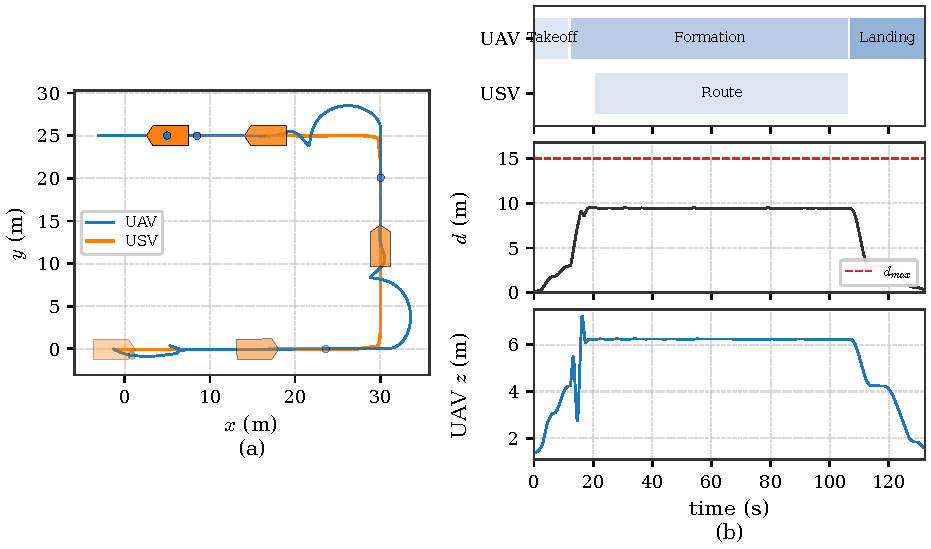
\includegraphics[width=\textwidth]{Results/figures/02_missions/scout.pdf}
    \caption[Scout mission.]{Scout mission: (a) paths of both vehicles, and (b) manoeuvres of each vehicle, separation $d$ and height of the \gls{uav}.}
    \label{fig:res_scout}
\end{figure}

% How is the UAV brought ahead of the bow?
The transfer from the takeoff to the point ahead of the bow is given as a straight line covered in $5\,\text{s}$, rather than as a single point. Right after the takeoff the tether is only $3\,\text{m}$ long, and a single point would ask the separation to grow faster than the winch pays out the tether. As in the first step of Section~\ref{subsec:res_tracking_tether}, the \gls{nmpc} would then keep within the pay-out rate by trading height for it, and bring the \gls{uav} down close to the deck. Covered in $5\,\text{s}$, the transfer climbs smoothly to its height, with a tilt below $14^\circ$, while the separation grows at up to $2.4\,\text{m/s}$, close to the pay-out rate.

% Does the UAV keep ahead of the bow as the USV turns?
Along the route, the \gls{uav} keeps its place with a mean error of $5\,\text{cm}$, Figure~\ref{fig:res_scout}. The largest errors, of $17\,\text{cm}$, are at the turns, where the point ahead of the bow swings around the \gls{usv} as it turns, and the \gls{uav} follows it on the wide arcs seen in Figure~\ref{fig:res_scout}a. The separation stays at $9.5\,\text{m}$, and the \gls{uav} lands on the pad, $3\,\text{cm}$ from its centre, once the route is over.

\subsection{Inspection}
\label{subsec:res_inspection}

% What does the inspection ask of the two vehicles?
In the inspection, the \gls{uav} circles a tower standing in the water, $12$ by $13\,\text{m}$ at its base, at a radius of $13\,\text{m}$ from its centre and $12\,\text{m}$ high. A circle of this size is beyond the reach of the tether from any fixed point, so the mission depends on the \gls{usv}. The \gls{uav} takes off and flies in formation ahead of the bow while the \gls{usv} sails to the tower. When the \gls{usv} arrives, the \gls{uav} starts the circle, given as a reference fixed in the world, and the \gls{usv} starts to support it from the water.

\begin{figure}[htbp]
    \centering
    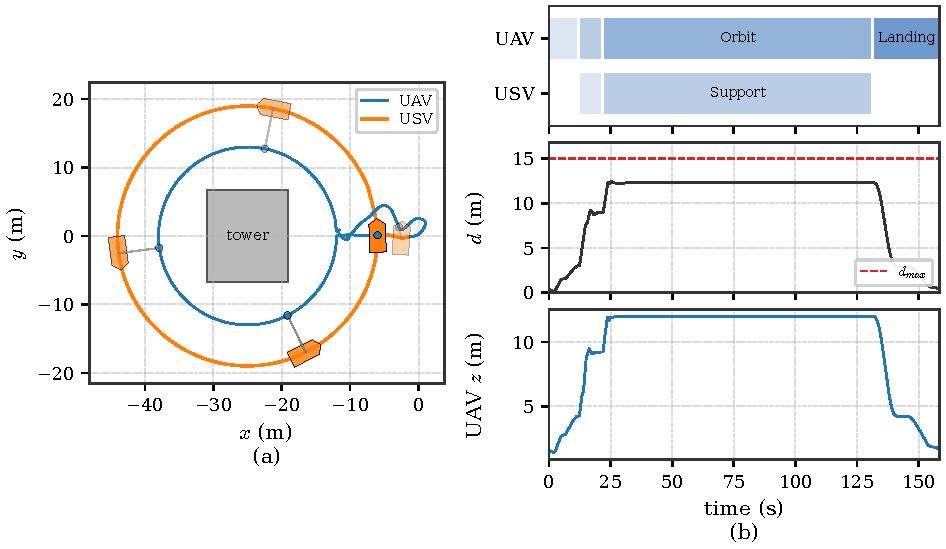
\includegraphics[width=\textwidth]{Results/figures/02_missions/inspection.pdf}
    \caption[Inspection mission.]{Inspection mission: (a) paths of both vehicles around the tower, and (b) manoeuvres of each vehicle, separation $d$ and height of the \gls{uav}.}
    \label{fig:res_inspection}
\end{figure}

% Does the support keep the UAV within reach?
Figure~\ref{fig:res_inspection} shows that the \gls{usv} keeps itself on the water below the \gls{uav}, $6\,\text{m}$ further from the tower, and follows it around the whole circle, at a radius that stays within $3\,\text{cm}$ of the intended $19\,\text{m}$. The separation stays at $12.3\,\text{m}$ throughout the lap, so that the \gls{uav} never comes close to the limit of the tether, and follows its circle with an error of $1\,\text{cm}$. The manoeuvres themselves are simple. The \gls{uav} follows a circle fixed in the world, regardless of the \gls{usv}, and the \gls{usv} follows the \gls{uav}, so that the two together cover a circle that neither could cover alone. The lap takes $110\,\text{s}$, after which the \gls{uav} lands on the pad, $4\,\text{cm}$ from its centre.

\subsection{Patrol}
\label{subsec:res_patrol}

% What happens in the patrol?
In the patrol, the \gls{usv} sails a route while the \gls{uav} orbits it, $7\,\text{m}$ away and $10\,\text{m}$ high, looking down. Near the route, a second vessel patrols a forbidden zone, and flees when either vehicle comes within $15\,\text{m}$ of it. The \gls{uav} detects it once it enters the field of view of its camera, assumed to be $120^\circ$ wide, which at this height reaches about $17\,\text{m}$ to each side, before the target notices it. From then on, the reference of the \gls{uav} is simply the point above the target, wherever it is, and the \gls{usv} pursues it.

\begin{figure}[htbp]
    \centering
    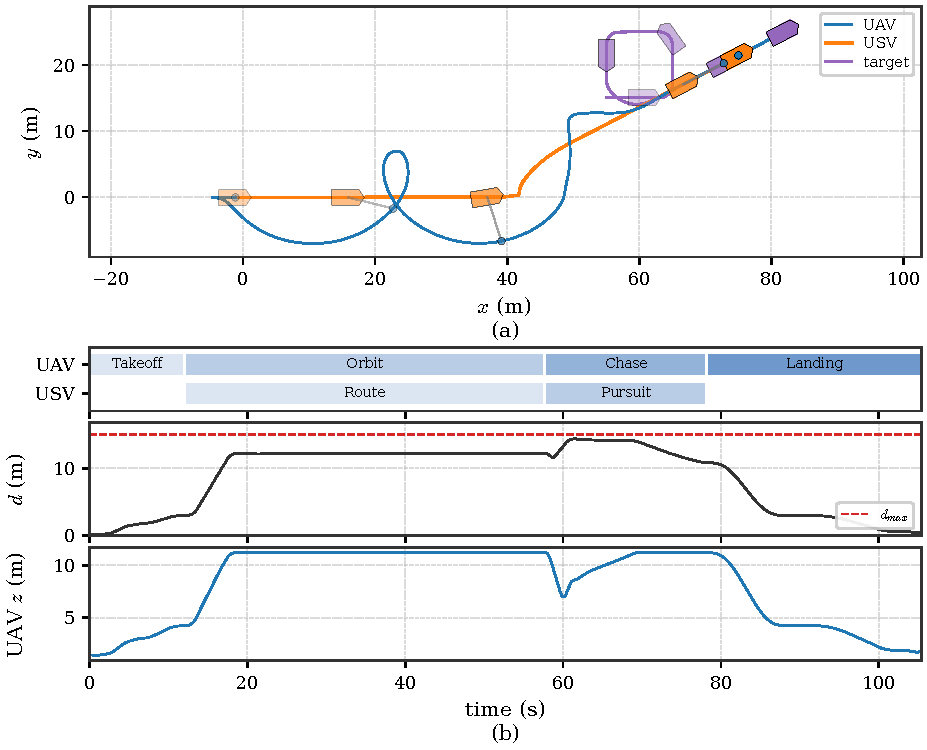
\includegraphics[width=\textwidth]{Results/figures/02_missions/patrol.pdf}
    \caption[Patrol mission.]{Patrol mission: (a) paths of both vehicles and of the target, and (b) manoeuvres of each vehicle, separation $d$ and height of the \gls{uav}.}
    \label{fig:res_patrol}
\end{figure}

% How does the UAV reach a target beyond the reach of the tether?
The target is detected $56\,\text{s}$ after the takeoff, $19\,\text{m}$ from the \gls{uav} and $23\,\text{m}$ from the \gls{usv}, beyond the reach of the tether, as shown in Figure~\ref{fig:res_patrol}. The reference above it is therefore brought within reach, along the line from the \gls{usv}, which also lowers it, and the \gls{uav} drops from $10$ to $5\,\text{m}$ as it flies towards the target. The separation reaches $14.7\,\text{m}$, within its limit. The \gls{uav} is above the target $5\,\text{s}$ after the detection, and as the \gls{usv} closes in, at up to $2.2\,\text{m/s}$ against the $1.5\,\text{m/s}$ of the fleeing target, the reference comes within reach and the \gls{uav} climbs back to its height. The \gls{usv} catches up with the target $21\,\text{s}$ after the detection, and the \gls{uav} then lands on the pad, $5\,\text{cm}$ from its centre.

% Are the limits respected?
The chase starts with the largest jump of the reference in the missions, and the commanded tilt reaches its limit. The roll of the \gls{uav} then reaches $34^\circ$ for $0.4\,\text{s}$, above its limit, while the total tilt of the vehicle stays below that commanded. The roll and the pitch are measured about axes turned by the commanded yaw, and the yaw of the \gls{uav}, which turns towards the target at the same time, lags its command by up to $13^\circ$, so that part of the commanded pitch appears as roll. Both vehicles otherwise stay within their limits throughout the mission.
